\section{FEM}

\subsection{2D as weighted residuals}
The PDE of second order (strom form) along with the corresponding BCs form the BVP
\begin{equation*}
	-\frac{\partial }{\partial x}\left(a_x \frac{\partial \Phi}{\partial x}\right) - \frac{\partial }{\partial y}\left(\frac{\partial \Phi}{\partial y}\right) + \beta \Phi = f, (x,y) \in \Omega \subseteq R^2
\end{equation*}
\begin{equation*}
	\Phi(x,y) = p, (x,y) \in \partial_D\Omega
\end{equation*}
\begin{equation*}
	\left(a_x \frac{\partial \Phi}{\partial x}\cdot \vec{e_x} + a_y \frac{\partial \Phi}{\partial y} \cdot \vec{e_y}\right) \cdot \vec{n} = q, (x,y) \in \partial_N\Omega
\end{equation*}
\begin{equation*}
	\partial_D\Omega \cup \partial_N\Omega = \partial\Omega = \textrm{boundary}(\Omega)
\end{equation*}
where $\Omega$ is the computational domain, $\alpha$ and $\beta$ are constants representing the material properties, $f$ is a predefined source term, $\vec{n}$ is a normal outward unit vector at a certain point on the Neumann boundary, and $\Phi$ is an unknown function. \\

The method of weighted residuals (approximation to $0$) is used in order to abtain an equivalent integral form (weak form as it is first order) of the 2D BVP. With some (s)magic the equivalent integral form becomes:
\begin{equation*}
	\iint\limits_{\left(\Omega\right)} \nabla w_i \cdot \left(a_x \frac{\partial \Phi}{\partial x} \vec{e_x} + a_y \frac{\partial \Phi}{\partial y} \vec{e_y}\right) d\Omega + \iint\limits_{\left(\Omega\right)} w_i\beta\Phi d\Omega - \iint\limits_{\left(\Omega\right)} w_i f d\Omega  - \int\limits_{\left(\partial_N\Omega\right)} w_i \cdot q \cdot dl = 0
\end{equation*}
The name 'weak' comes from the fact that this form consists of only partial derivatives of first oder, while the partial derivatives in the BVP are of second order ('strong' form).

\subsubsection{Meshing}
The goal for meshing is to get from complex geometries to large numbers (max. 25 Million because of rounding errors) of elements with simple geometry (triangles, quadrilaterals).\newline

With a subdivison of
\begin{equation*}
	\Omega = \bigcup\limits_{e=1}^{N_e} \Omega^e
\end{equation*}
where the superscript $e$ refers to a local approximation within the element $e$, the original weak form becomes
\begin{equation*}
	\sum_{e=1}^{N_e} \iint\limits_{\left(\Omega^e\right)} \alpha^e \nabla {w_i}^e \cdot \nabla \Phi^e\,d\Omega + \sum_{e=1}^{N_e} \iint\limits_{\left(\Omega^e\right)} {w_i}^e\beta^e\Phi^e\,d\Omega - \sum_{e=1}^{N_e} \iint\limits_{\left(\Omega^e\right)}{w_i}^e f^e\,d\Omega  - \sum_{{\substack{e\\\partial \Omega ^e\in\partial_N\Omega}}} \int\limits_{\partial \Omega^e} {w_i}^e q^e\,dl = 0
\end{equation*} 

\begin{minipage}[rt]{12cm}
	\begin{tabular}{l}
		Linear approximation of the unknown function over the element: \\
		\(\displaystyle \Phi^e(x,y) = a + bx + cy \) \\
		Expressed wit respect to the nodal values: \\
		\(\displaystyle {\Phi_1}^e = a + b{x_1}^e + c{y_1}^2 \) \\
		\(\displaystyle {\Phi_2}^e = a + b{x_2}^e + c{y_2}^2 \) \\
		\(\displaystyle {\Phi_3}^e = a + b{x_3}^e + c{y_3}^2 \) \\
		\(\displaystyle \Rightarrow 
			\begin{bmatrix}
				{\Phi_1}^e \\
				{\Phi_2}^e \\
				{\Phi_3}^e
			\end{bmatrix} 
			=
			\begin{bmatrix}
				1 & {x_1}^e & {y_1}^e \\
				1 & {x_2}^e & {y_2}^e \\
				1 & {x_3}^e & {y_3}^e 
			\end{bmatrix}
			\cdot
			\begin{bmatrix}
				a \\
				b \\
				c
			\end{bmatrix}
			= 
			\begin{bmatrix}
				S^e 
			\end{bmatrix}
			\cdot 
			\begin{bmatrix}
				a \\
				b \\
				c
			\end{bmatrix} \) \\
	\end{tabular}
\end{minipage}
\begin{minipage}[lt]{8cm}
	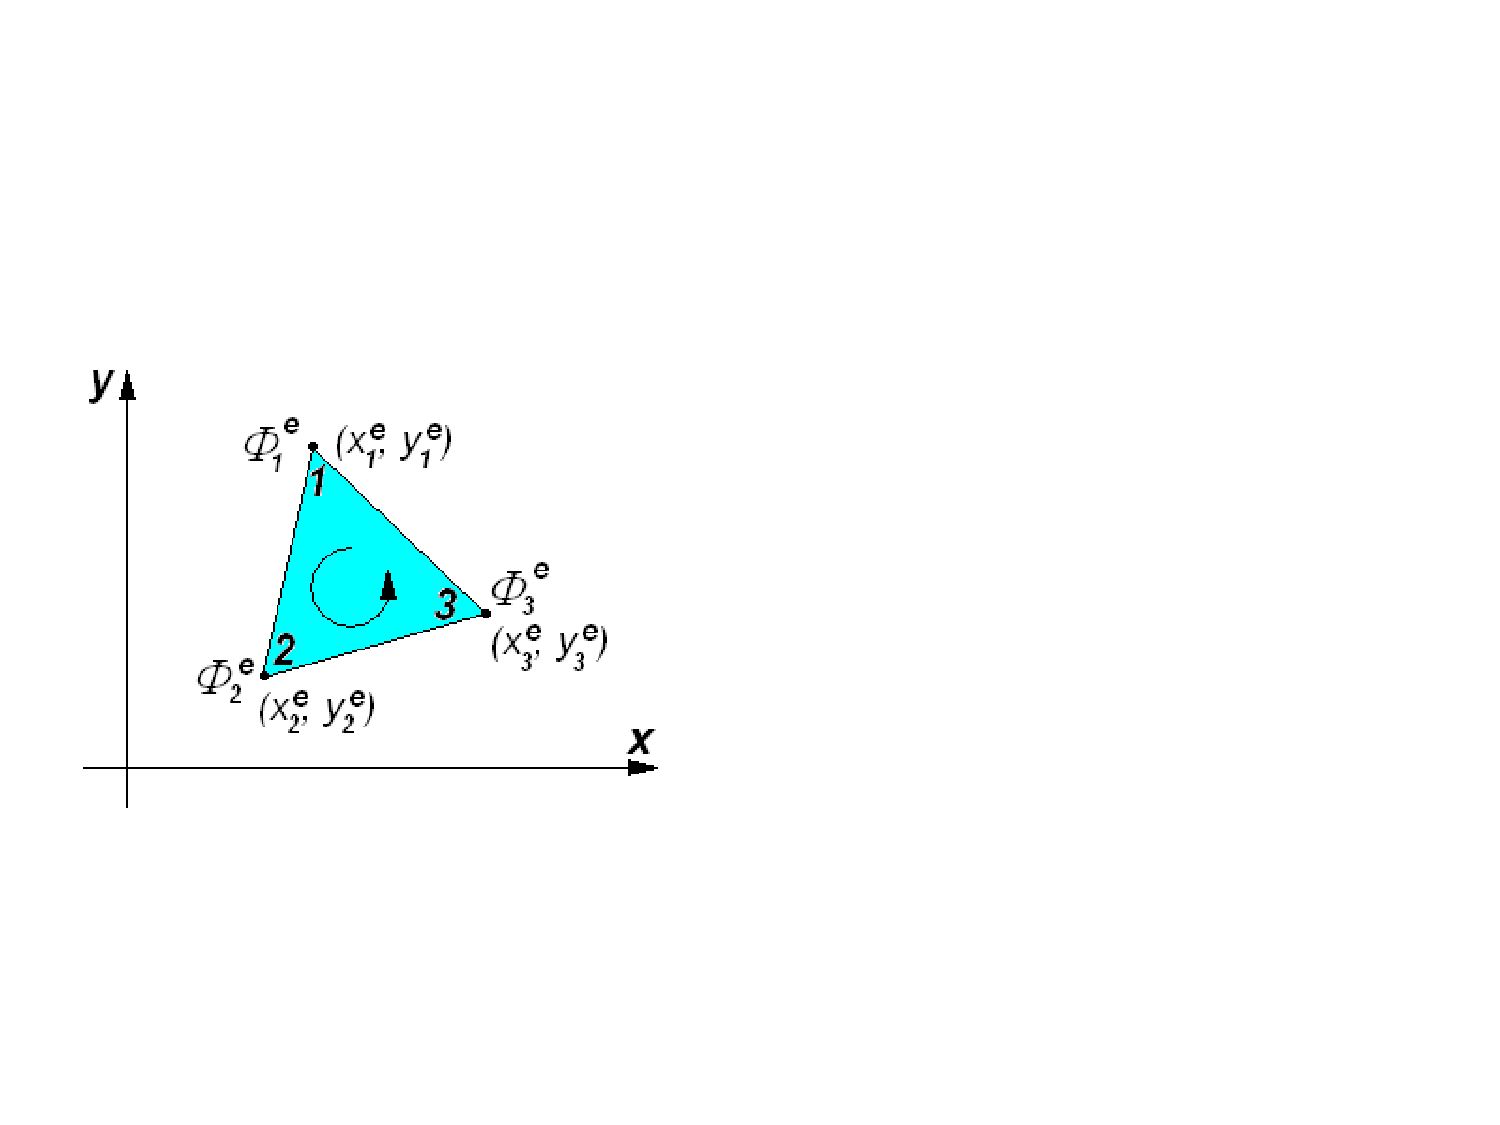
\includegraphics[width=.8\textwidth]{./images/nodes.pdf}\\
\end{minipage}
This system can be solved as
\begin{equation*}
	\begin{bmatrix}
		a \\
		b \\
		c
	\end{bmatrix}
	= 
	\begin{bmatrix}
		S^e
	\end{bmatrix}^{-1}
	\cdot
	\begin{bmatrix}
		{\Phi_1}^e \\
		{\Phi_2}^e \\
		{\Phi_3}^e
	\end{bmatrix}
\end{equation*}
The inversion of the matrix $\begin{bmatrix}S^e\end{bmatrix}$ is given as
\begin{equation*}
	\begin{bmatrix}
		S^e
	\end{bmatrix}^{-1}
	= 
	\begin{bmatrix}
		1 & {x_1}^e & {y_1}^e \\
		1 & {x_2}^e & {y_2}^e \\
		1 & {x_3}^e & {y_3}^e 
	\end{bmatrix}^{-1}
	= \frac{1}{2A}
	\begin{bmatrix}
		{x_2}^e {y_3}^e - {x_3}^e{y_2}^e & {x_3}^e {y_1}^e - {x_1}^e{y_3}^e & {x_1}^e {y_2}^e - {x_2}^e{y_1}^e \\
		{y_2}^e - {y_3}^e & {y_3}^e - {y_1}^e & {y_1}^e - {y_2}^e \\
		{x_3}^e - {x_2}^e & {x_1}^e - {x_3}^e & {x_2}^e - {x_1}^e \\
 	\end{bmatrix}
\end{equation*}
where 'A' is the surface area of the triangular element
\begin{equation*}
	A = \frac{1}{2} \left[\left({x_2}^e - {x_1}^e\right) \cdot \left({y_3}^e - {y_1}^e\right) - \left({x_3}^e - {x_1}^e\right) \cdot \left({y_2}^e - {y_1}^e\right) \right]
\end{equation*}
which should be as large as possible. Finally, the approximation of the unknown function becomes
\begin{equation*}
	\Phi^e(x,y) =
	\begin{bmatrix}
		1 & x & y
	\end{bmatrix}
	\cdot 
	\begin{bmatrix}
		S^e
	\end{bmatrix}^{-1}
	\cdot
	\begin{bmatrix}
		{\Phi_1}^e \\
		{\Phi_2}^e \\
		{\Phi_2}^e \\
	\end{bmatrix}
	=
	\begin{bmatrix}
		{N_1}^e(x,y) & {N_2}^e(x,y) & {N_2}^e(x,y)
	\end{bmatrix}
	\cdot 
	\begin{bmatrix}
		{\Phi_1}^e \\
		{\Phi_2}^e \\
		{\Phi_2}^e \\
	\end{bmatrix}
	= \sum_{i=1}^{3} {N_i}^e(x,y) \cdot {\Phi_i}^e
\end{equation*}
where ${N_i}^e(x,y)$ is the shape function of the node $i$ of the element $e$.

\textbf{\\ \\ Shape function \\}
The shape functions of linear triangular elements are obtained as
\begin{equation*}
	{N_1}^e(x,y) = \frac{1}{2A} \left[\underbrace{\left({x_2}^e {y_3}^e - {x_3}^e {y_2}^e\right)}_{a_1} +  \underbrace{\left({y_2}^e - {y_3}^e\right)}_{b_1} \cdot x + \underbrace{\left({x_3}^e - {x_2}^e\right)}_{c_1} \cdot y\right]
\end{equation*}
\begin{equation*}
	{N_2}^e(x,y) = \frac{1}{2A} \left[\underbrace{\left({x_3}^e {y_1}^e - {x_1}^e {y_3}^e\right)}_{a_2} +  \underbrace{\left({y_3}^e - {y_1}^e\right)}_{b_2}\cdot x + \underbrace{\left({x_1}^e - {x_3}^e\right)}_{c_2} \cdot y\right]
\end{equation*}
\begin{equation*}
	{N_3}^e(x,y) = \frac{1}{2A} \left[\underbrace{\left({x_1}^e {y_2}^e - {x_2}^e {y_1}^e\right)}_{a_3} +  \underbrace{\left({y_1}^e - {y_2}^e\right)}_{b_3} \cdot x + \underbrace{\left({x_2}^e - {x_1}^e\right)}_{c_3} \cdot y\right]
\end{equation*}

\begin{figure}[h!]
	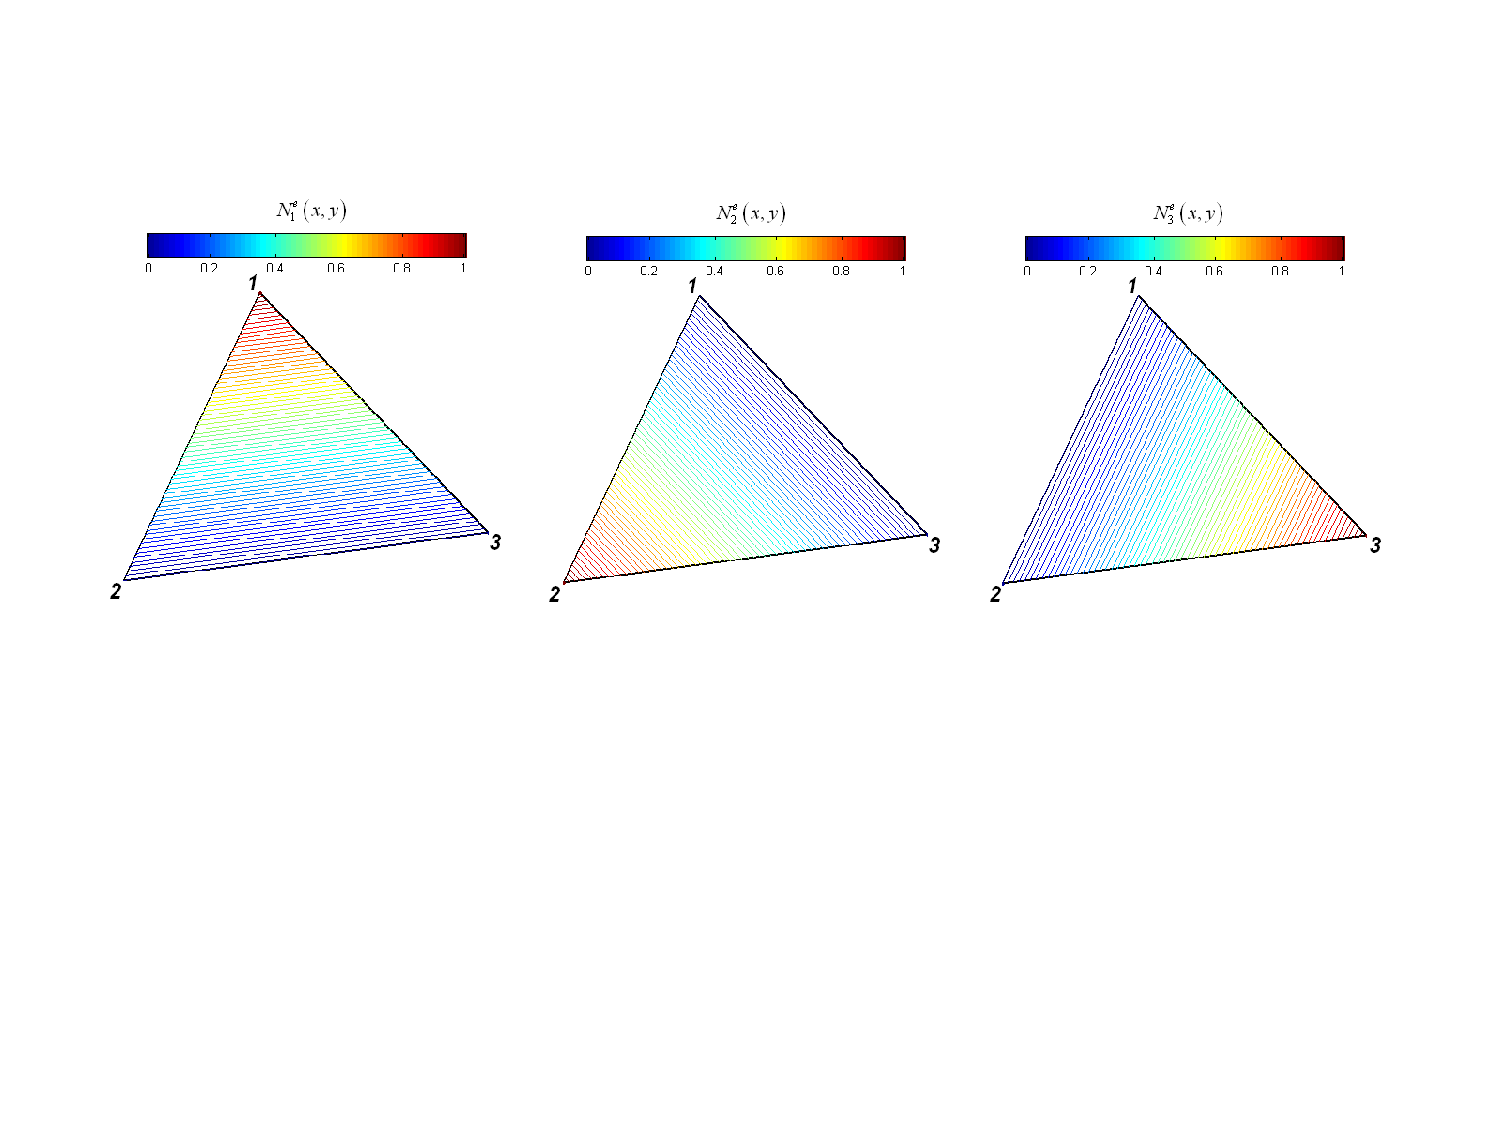
\includegraphics[width=.8\textwidth]{./images/shapeFunc.pdf}
\end{figure}

Due to local character of the shape function, it is simple to switch from the local (element based) notation to the global (computational domain) notation:
\begin{equation*}
	\Phi^e(x,y) = \sum_{i=1}^{3}{N_i}^e(x,y) \cdot {\Phi_i}^e \xrightarrow{\textrm{Local to Global Notation}} \Phi(x,y) = \sum_{i=1}^{N_n} N_i(x,y) \cdot \Phi_i
\end{equation*}

\subsubsection{Sparse Linear System}
\begin{minipage}[lt]{13cm}
	Galerkin method suggests that the shape functions themselves play a role of the weigthing functions: 
	\begin{equation*}
		w_i(x,y) = N_i(x,y)
	\end{equation*}
	which leads to a linear system 
	\begin{equation*}	
		\left[K\right] \cdot \underbrace{\{\Phi\}}_{\textrm{unknowns}} = \underbrace{\{b\}}_{\textrm{source}}
	\end{equation*}
	It is evident that each element contributes to the matrix and to the right-hand side. 
\end{minipage}
\begin{minipage}[rt]{7cm}
	\begin{centering}
		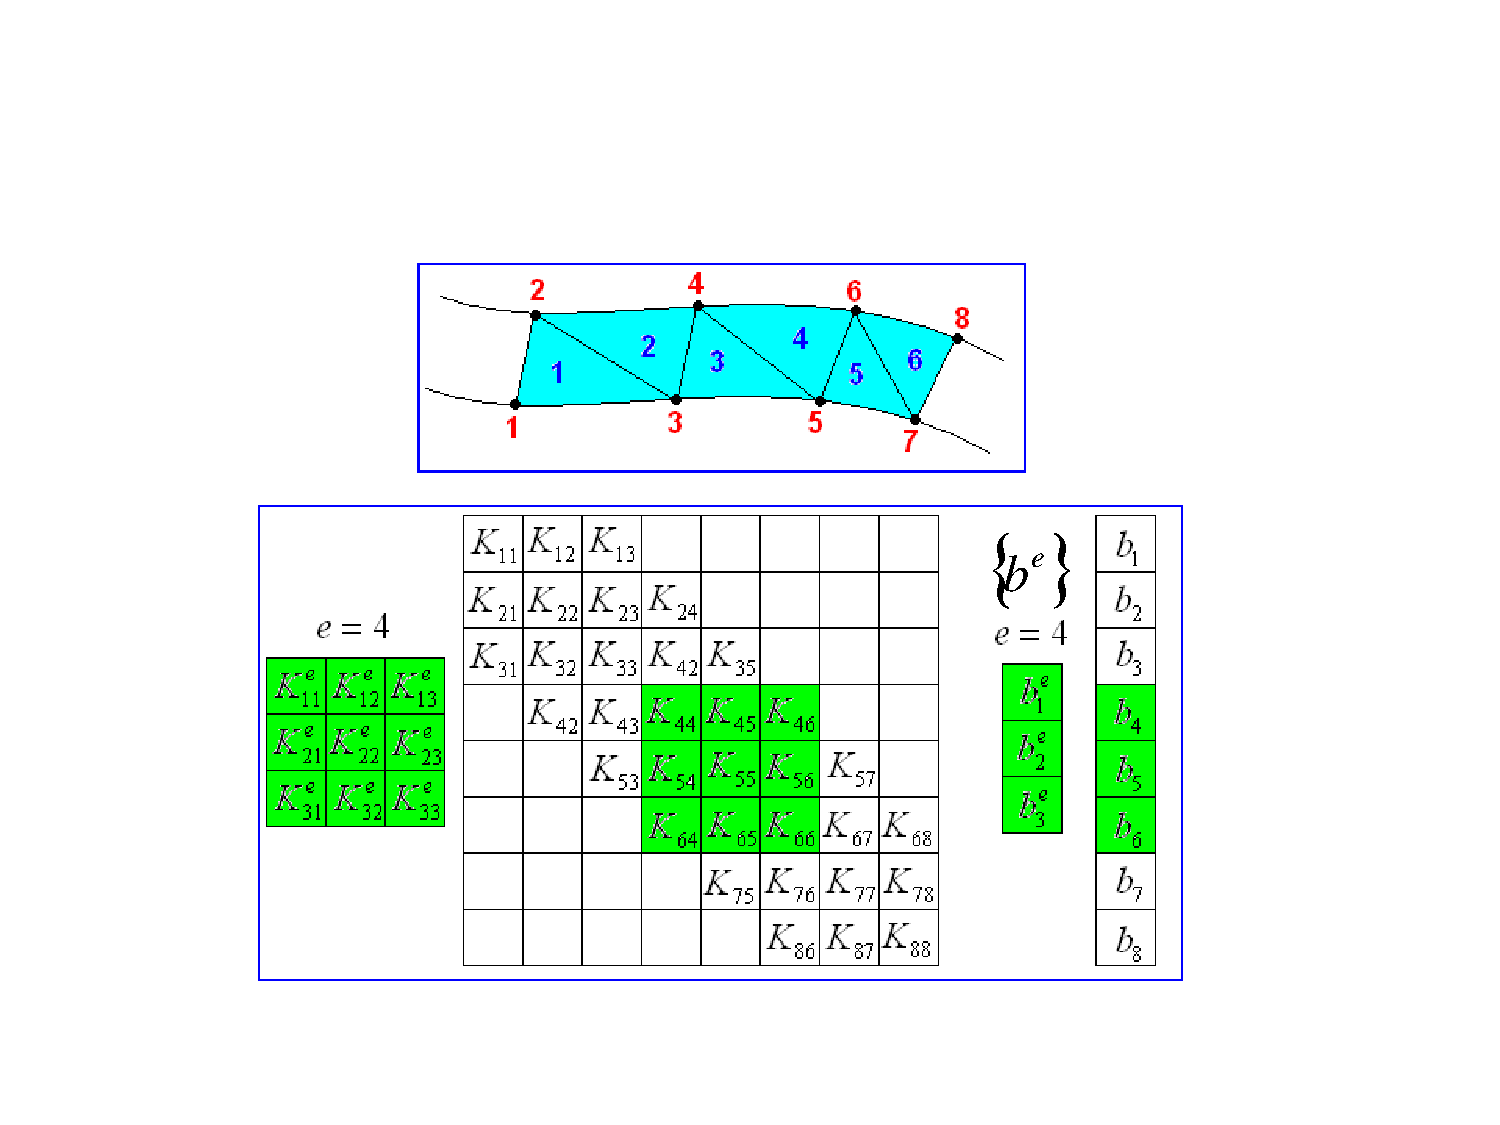
\includegraphics[width=.85\textwidth]{./images/sparse.pdf}
	\end{centering}
\end{minipage}

\textbf{\\ \\Solvers \\}
Direct solution of the FEM System of equations
\begin{itemize}
	\item LU-decompositon
	\item Cholesky factorization
	\item Direct methods are impractical for large systems (above $10^6$ unknowns) due to ist high number of mathematical operations and round-off error
\end{itemize}
Iterative solution methods
\begin{itemize}
	\item CG
	\item BiCG
	\item GMRES (best for 3D)
	\item Iterative methods are very suitable for large systems but have a slow convergence when the FEM matrix is ill-conditioned (which is usually the case)
	\item Convergence acceleration could be achieved by using preconditioning methods: diagonal preconditioning, ILU (incomplete-LU), ect. 
\end{itemize}

\subsection{3D as variational integral (integral of electric energy)}
The energy in a system can be computed as
\begin{equation*}
	W_e = \frac{1}{2} \iiint\limits_{\left(\Omega\right)} \rho \cdot \varphi \cdot dV = \frac{1}{2} \iiint\limits_{\left(\Omega	\right)} \vec{D} \cdot \vec{E}\,dV
\end{equation*}
(first integral is the microscopic pendent to the macroscopic $W_e = \frac{1}{2} QU = \frac{1}{2}CU^2$) \newline
Since a physical system is always trying to minimize its energy, the so-called FEM variational integral can be written as
\begin{equation*}
	\textrm{min: } W_e = \iiint\limits_{\left(\Omega\right)} \rho \cdot \varphi \cdot dV - \frac{1}{2} \iiint\limits_{\left(\Omega\right)} \varepsilon \cdot \left(\nabla \varphi\right)^2 dV
\end{equation*}

\begin{minipage}[rt]{12cm}
	\begin{tabular}{l}
		Linear tetrahedral element: \\
		\begin{equation*}
			\Phi^e(x,y,z) = \sum_{k=1}^{4}{N_k}^e(x,y,z) \cdot {\Phi_k}^e
		\end{equation*} \\
		With the shape function: \\
		\begin{equation*}
			{N_k}^e = (x,y,z) = \frac{1}{6 V^e}\left({a_j}^e + {b_j}^e x + {c_j}^e y + {d_j}^e z\right)
		\end{equation*}
	\end{tabular}
\end{minipage}
\begin{minipage}[lt]{8cm}
	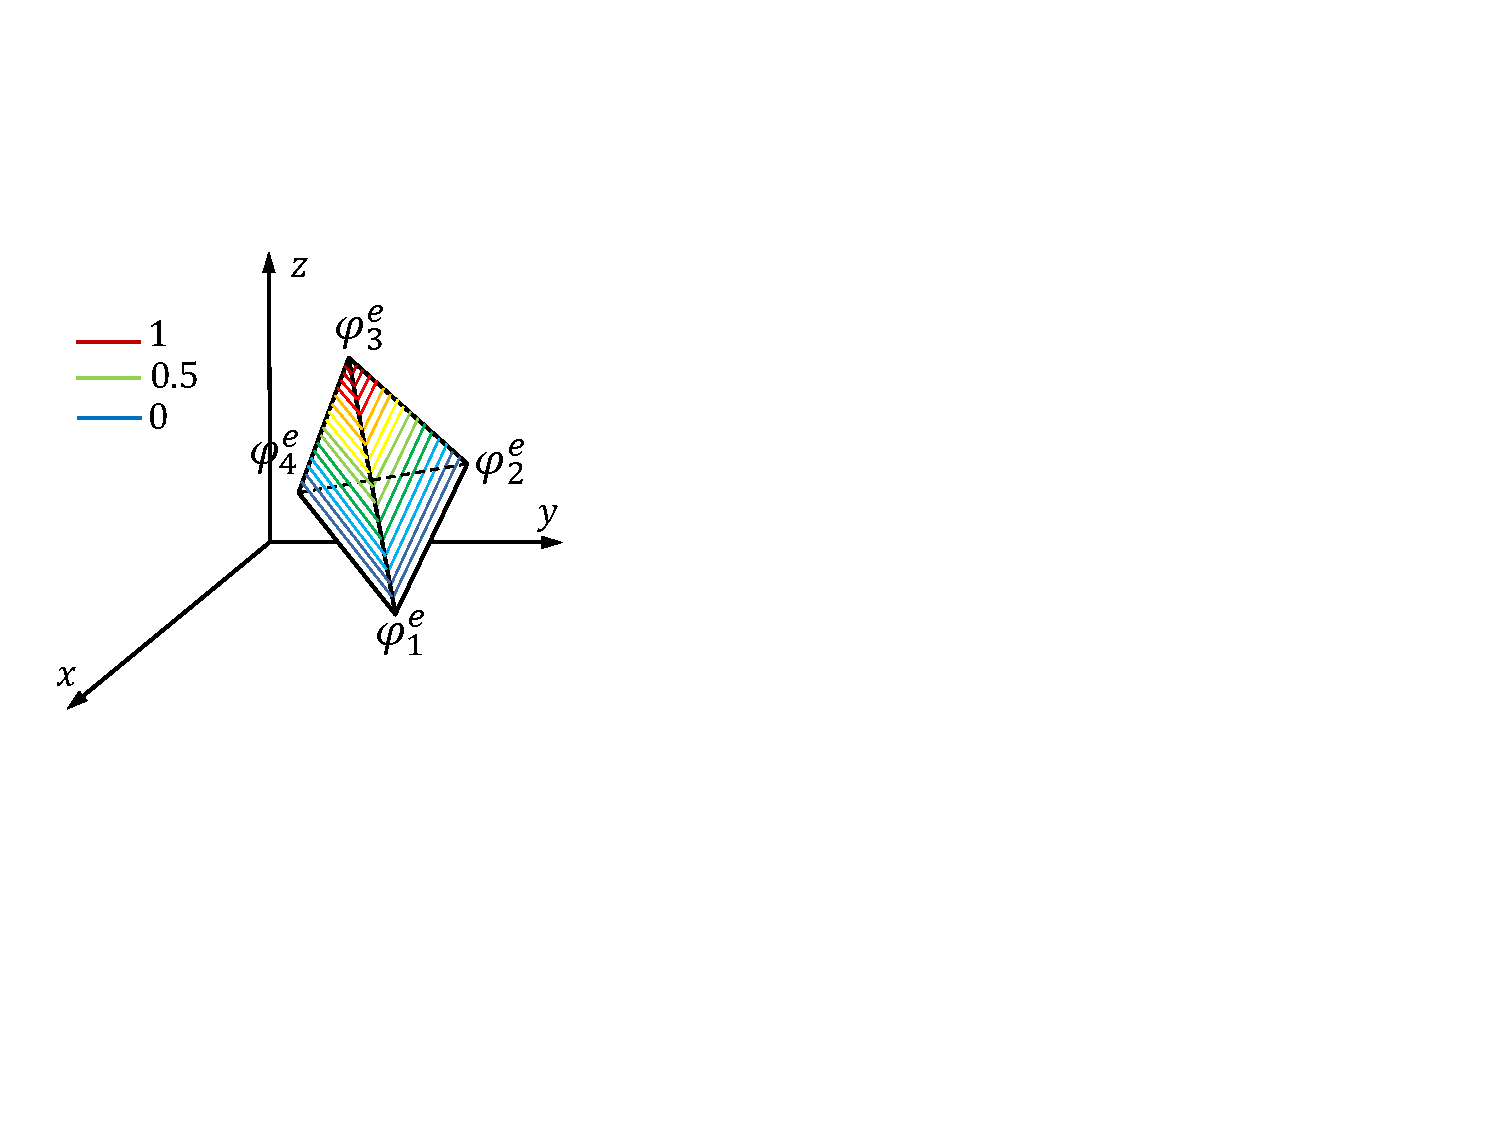
\includegraphics[width=.6\textwidth]{./images/tetraheder.pdf}\\
\end{minipage}

\subsubsection{Sparse system of linear equations}
Again a large sparse system with the following form
\begin{equation*}	
	\underbrace{\left[K\right]}_{\textrm{sparse matrix}} \cdot \underbrace{\{\Phi\}}_{\textrm{unknowns}} = \underbrace{\{E\}}_{\textrm{excitation}}
\end{equation*}
is obtained, with the vectors:
\begin{equation*}
	K_{kl} = \sum_{\substack{e\\k,l\in\Omega^e}} \iiint\limits_{\left(\Omega ^e\right)} \varepsilon \cdot \nabla N_k(x,y,z) \cdot \nabla N_l(x,y,z) \cdot dV
	\hspace{2cm}
	\{\Phi\} =
	\begin{bmatrix}
		\varphi_1 \\
		\varphi_2 \\ 
		\vdots \\
		\varphi_N
	\end{bmatrix}
\end{equation*}
\begin{equation*}
	E_l = \sum_{\substack{e\\l\in\Omega^e}} \iiint\limits_{\left(\Omega ^e\right)} \rho \cdot N_l(x,y,z) \cdot dV
\end{equation*}
where $k$ is the column and $l$ the row of the sparse matrix $K$. \newline \newline
\textbf{Important:} BC are set in $K$:
\begin{itemize}
	\item Dirichlet: row = 0, exept diagonal elements
	\item Neumann: this is already set to 0
\end{itemize}

\subsection{Vector form}
Nodal elements give contuinity in tangential and normal components, vectors only in tangential component. Eddy current simulations for example will deliver wrong results if nodal elemnts are used. \newline \newline

A vector weak form approach for solving eddy current problems is given as
\begin{equation*}
	\iint\limits_{\left(\Omega\right)} \left(\frac{1}{\mu}\nabla \times \vec{A}\right) \cdot \left(\nabla \times \vec{w}_i\right)\,dS + \iint\limits_{\left(\Omega\right)} \vec{w}_i \cdot j\omega\sigma\vec{A}\,dS = \iint\limits_{\left(\Omega\right)}\vec{w}_i \cdot \vec{J}_s\,dS
 \end{equation*}
 The vector functions used for approximating the vector unknown function over a single element are
 \begin{equation*}
 	\vec{A}^e\left(x,y\right) = \sum_{j=1}^{3}\vec{N_j}^e\left(x,y\right) {A_j}^e, {A_j}^e = \vec{e_j}^e \cdot \vec{A} \xrightarrow{\textrm{Local to Global Notation}} \vec{A}\left(x,y\right) = \sum_{j=1}^{N_{\textrm{edges}}} \vec{N}_j \left(x,y\right) A_j, Aj = \vec{e}_j \cdot \vec{A}
 \end{equation*}
 where each edge belongs to two elements (or one if Boundary Condition!).
 \begin{figure}[h!]
	 \centering
	 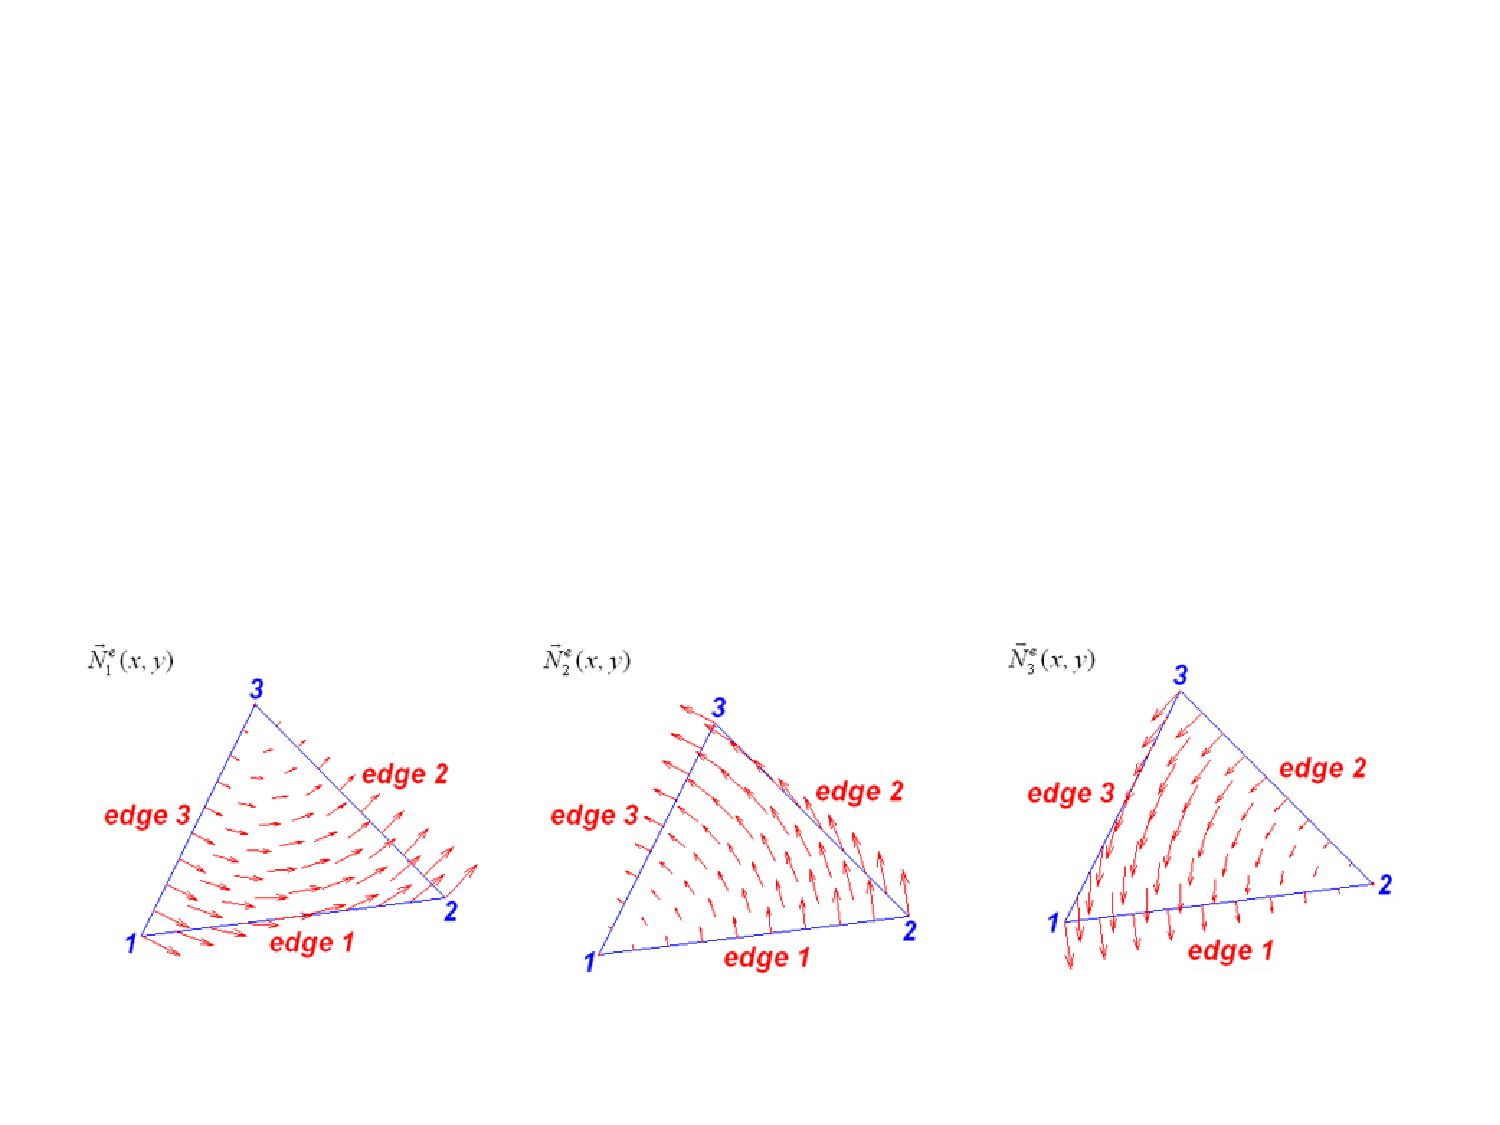
\includegraphics[width=.8\textwidth]{./images/vectorShape.pdf}
 \end{figure}
 
Choosing the weighting function the same as the vector shape function (Galerkin approach), the linear system
\begin{equation*}
	\left[K\right] \cdot \{A\} = \{b\}
\end{equation*}
can be solved with the vectors
\begin{equation*}
	K_{ij} = \sum_{\substack{e\\i,j\in\Delta^e}} \left(\iint\limits_{\left(\Delta^e\right)} \frac{1}{\mu} \underbrace{\left(\nabla \times \vec{N}_i\right)\cdot \left(\nabla \times \vec{N}_j\right)}_{\textrm{bad conditioned}}\,dS + \iint\limits_{\left(\Delta^e\right)} j\omega\sigma\vec{N}_i\cdot \vec{N}j\,dS\right)
	\hspace{2cm}
	b_i = \sum_{i\in\Delta^e}^{\textrm{Elements}} \iint\limits_{\Delta^e} \vec{N}_i \cdot \vec{J}_s\,dS.
\end{equation*}